\documentclass{beamer}
\usetheme{CENIDETDIE}
\setbeamertemplate{caption}[numbered]
\usefonttheme[onlymath]{serif}

% ------------------------------------------------------------------------------------------------

\usepackage[utf8]{inputenc}
\usepackage[T1]{fontenc}
\usepackage{helvet}
\usepackage{graphicx} % Allows including images
\usepackage{booktabs} % Allows the use of \toprule, \midrule and \bottomrule tables
\usepackage{amsmath}
\usepackage{color}
\usepackage{hyperref}
\usepackage{subfig}
%\usepackage{showframe}
\usepackage[absolute,overlay]{textpos} %To place the images
\usepackage[document]{ragged2e}
%\usepackage{authblk} %many authors
\numberwithin{figure}{section}
%\numberwithin{equation}{section}
\usepackage{natbib}
\usepackage{multirow}

% ------------------------------------------------------------------------------------------------

\title{\textbf{ \textit{Simplest Fermion Vector-Like Portal Dark Matter model:}}}
\subtitle{{\small 	Search in the compressed mass region at the CMS experiment}}
\author[C.Salazar]{\textbf{Camilo Salazar} }
\institute[UdeA]{camilo.salazar@cern.ch}

%\author{\textit{\textbf{Camilo A Salazar G}}}
%\institute{\url{camilo.salazar@cern.ch} }
\date{\today}


% ------------------------------------------------------------------------------------------------

\begin{document}

% ------------------------------------------------------------------------------------------------

\begin{frame}[plain,t]
\titlepage
\end{frame}


% ------------------------------------------------------------------------------------------------

\begin{frame}[plain,noframenumbering]
  \addtocounter{framenumber}{-1}
  \scriptsize
%   \thispagestyle{empty}
  \frametitle{Contenido}
  \setbeamertemplate{section in toc}[sections numbered]
  \tableofcontents[hideallsubsections]
\end{frame}

% ------------------------------------------------------------------------------------------------

\section{Introduction}
\begin{frame}
\frametitle{Introduction}
\justifying{
	
	
	Dark Matter (DM) constitutes one of the main unsolved problems in fundamental physics. 
	Ever since it was proposed to explain the rotation curves of galaxies, 
	some other astronomical observations left little doubt of its existence.
	\vspace{5 mm}
	
	Whatever DM is, the Standard Model (SM) is not able to produce a candidate that have, at the present time in 
	the universe, stability and also interact very little or not at all with known matter, proven properties of DM. 

}


\end{frame}

% ------------------------------------------------------------------------------------------------

\begin{frame}
\frametitle{Rotational Velocities}


\begin{figure}[!tbp]
	\centering
	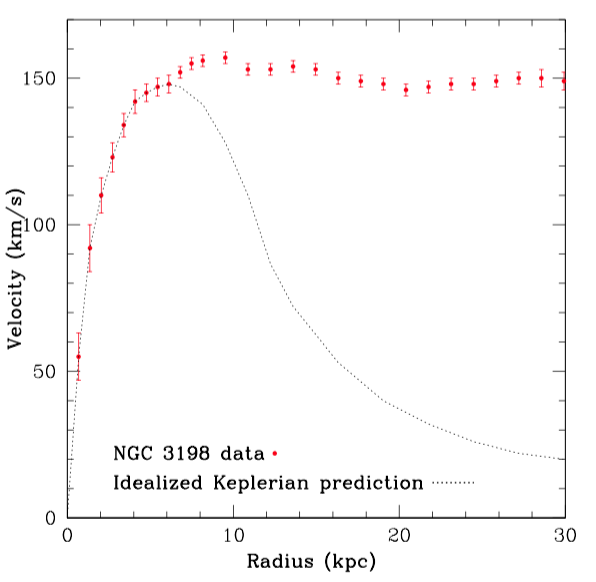
\includegraphics[width=0.6\textwidth]{pictures/fig_Introduction_rotation_curve_1}\label{fig:f1}
	\caption{Measured rotational velocities of HI regions in NGC 3198 compared to an idealized Keplerian behavior [Astron. and Astrophys. 223, 47-60]}
\end{figure}

\end{frame}

% ------------------------------------------------------------------------------------------------

\begin{frame}
\frametitle{Bullet cluster}


\begin{figure}[!tbp]
	\centering
	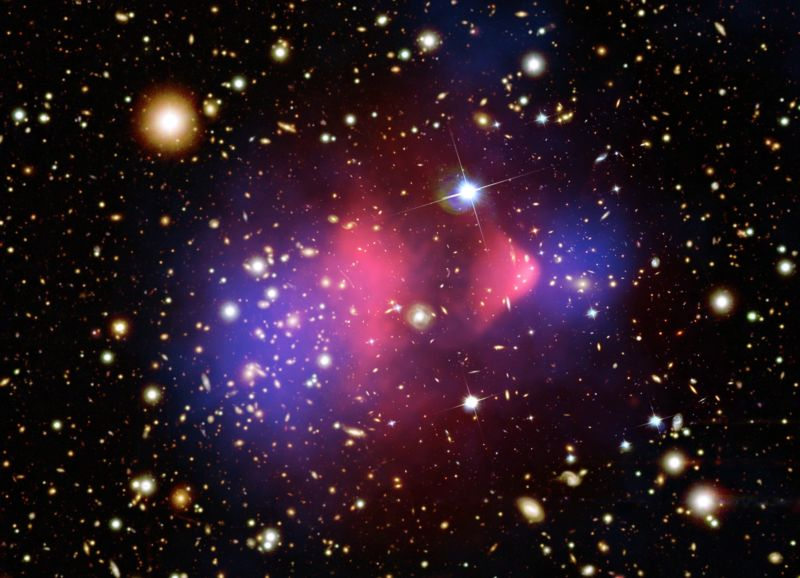
\includegraphics[width=0.8\textwidth]{pictures/bulletcluster}\label{fig:f1}
	\caption{The Bullet cluster, the result of a subcluster (the “bullet”) colliding with the larger galaxy cluster 1E 0657-56  [arXiv:1711.02117]}
\end{figure}

\end{frame}

% ------------------------------------------------------------------------------------------------


\section{Motivation}
\begin{frame}
\frametitle{Motivation}

\begin{figure}[!tbp]
	\centering
	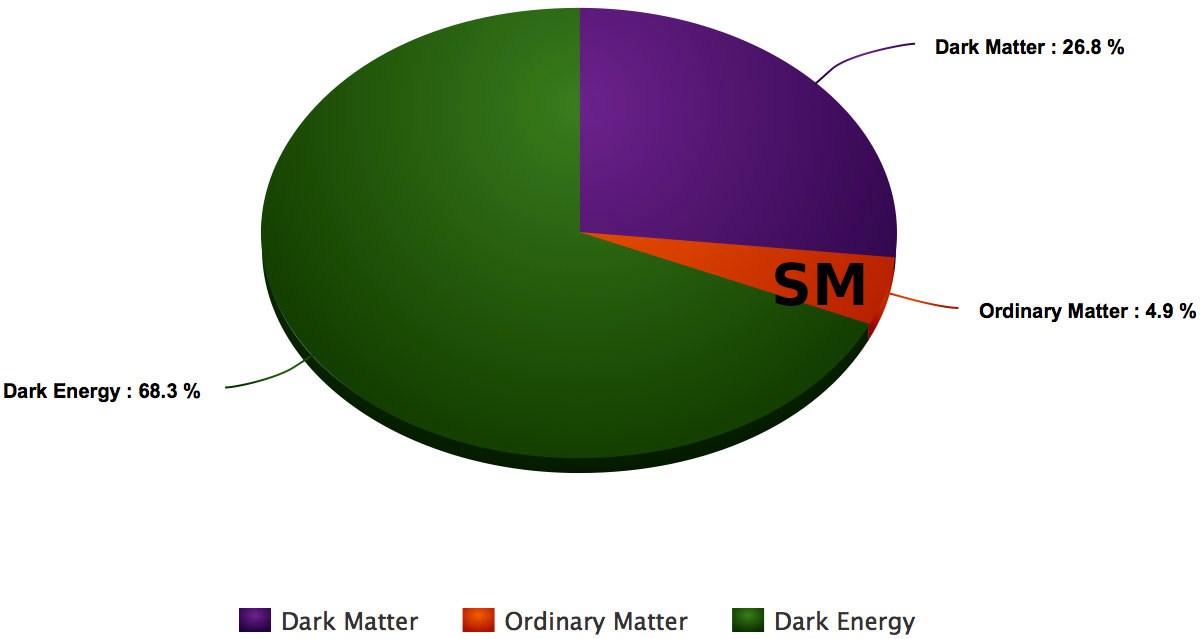
\includegraphics[width=0.9\textwidth]{pictures/pie}\label{fig2}
	\caption{{\scriptsize Simplified plot showing the estimate abundances}}
	
\end{figure}

\end{frame}

% ------------------------------------------------------------------------------------------------

\begin{frame}
\frametitle{Detection Channels}

\begin{figure}[!tbp]
	\centering
	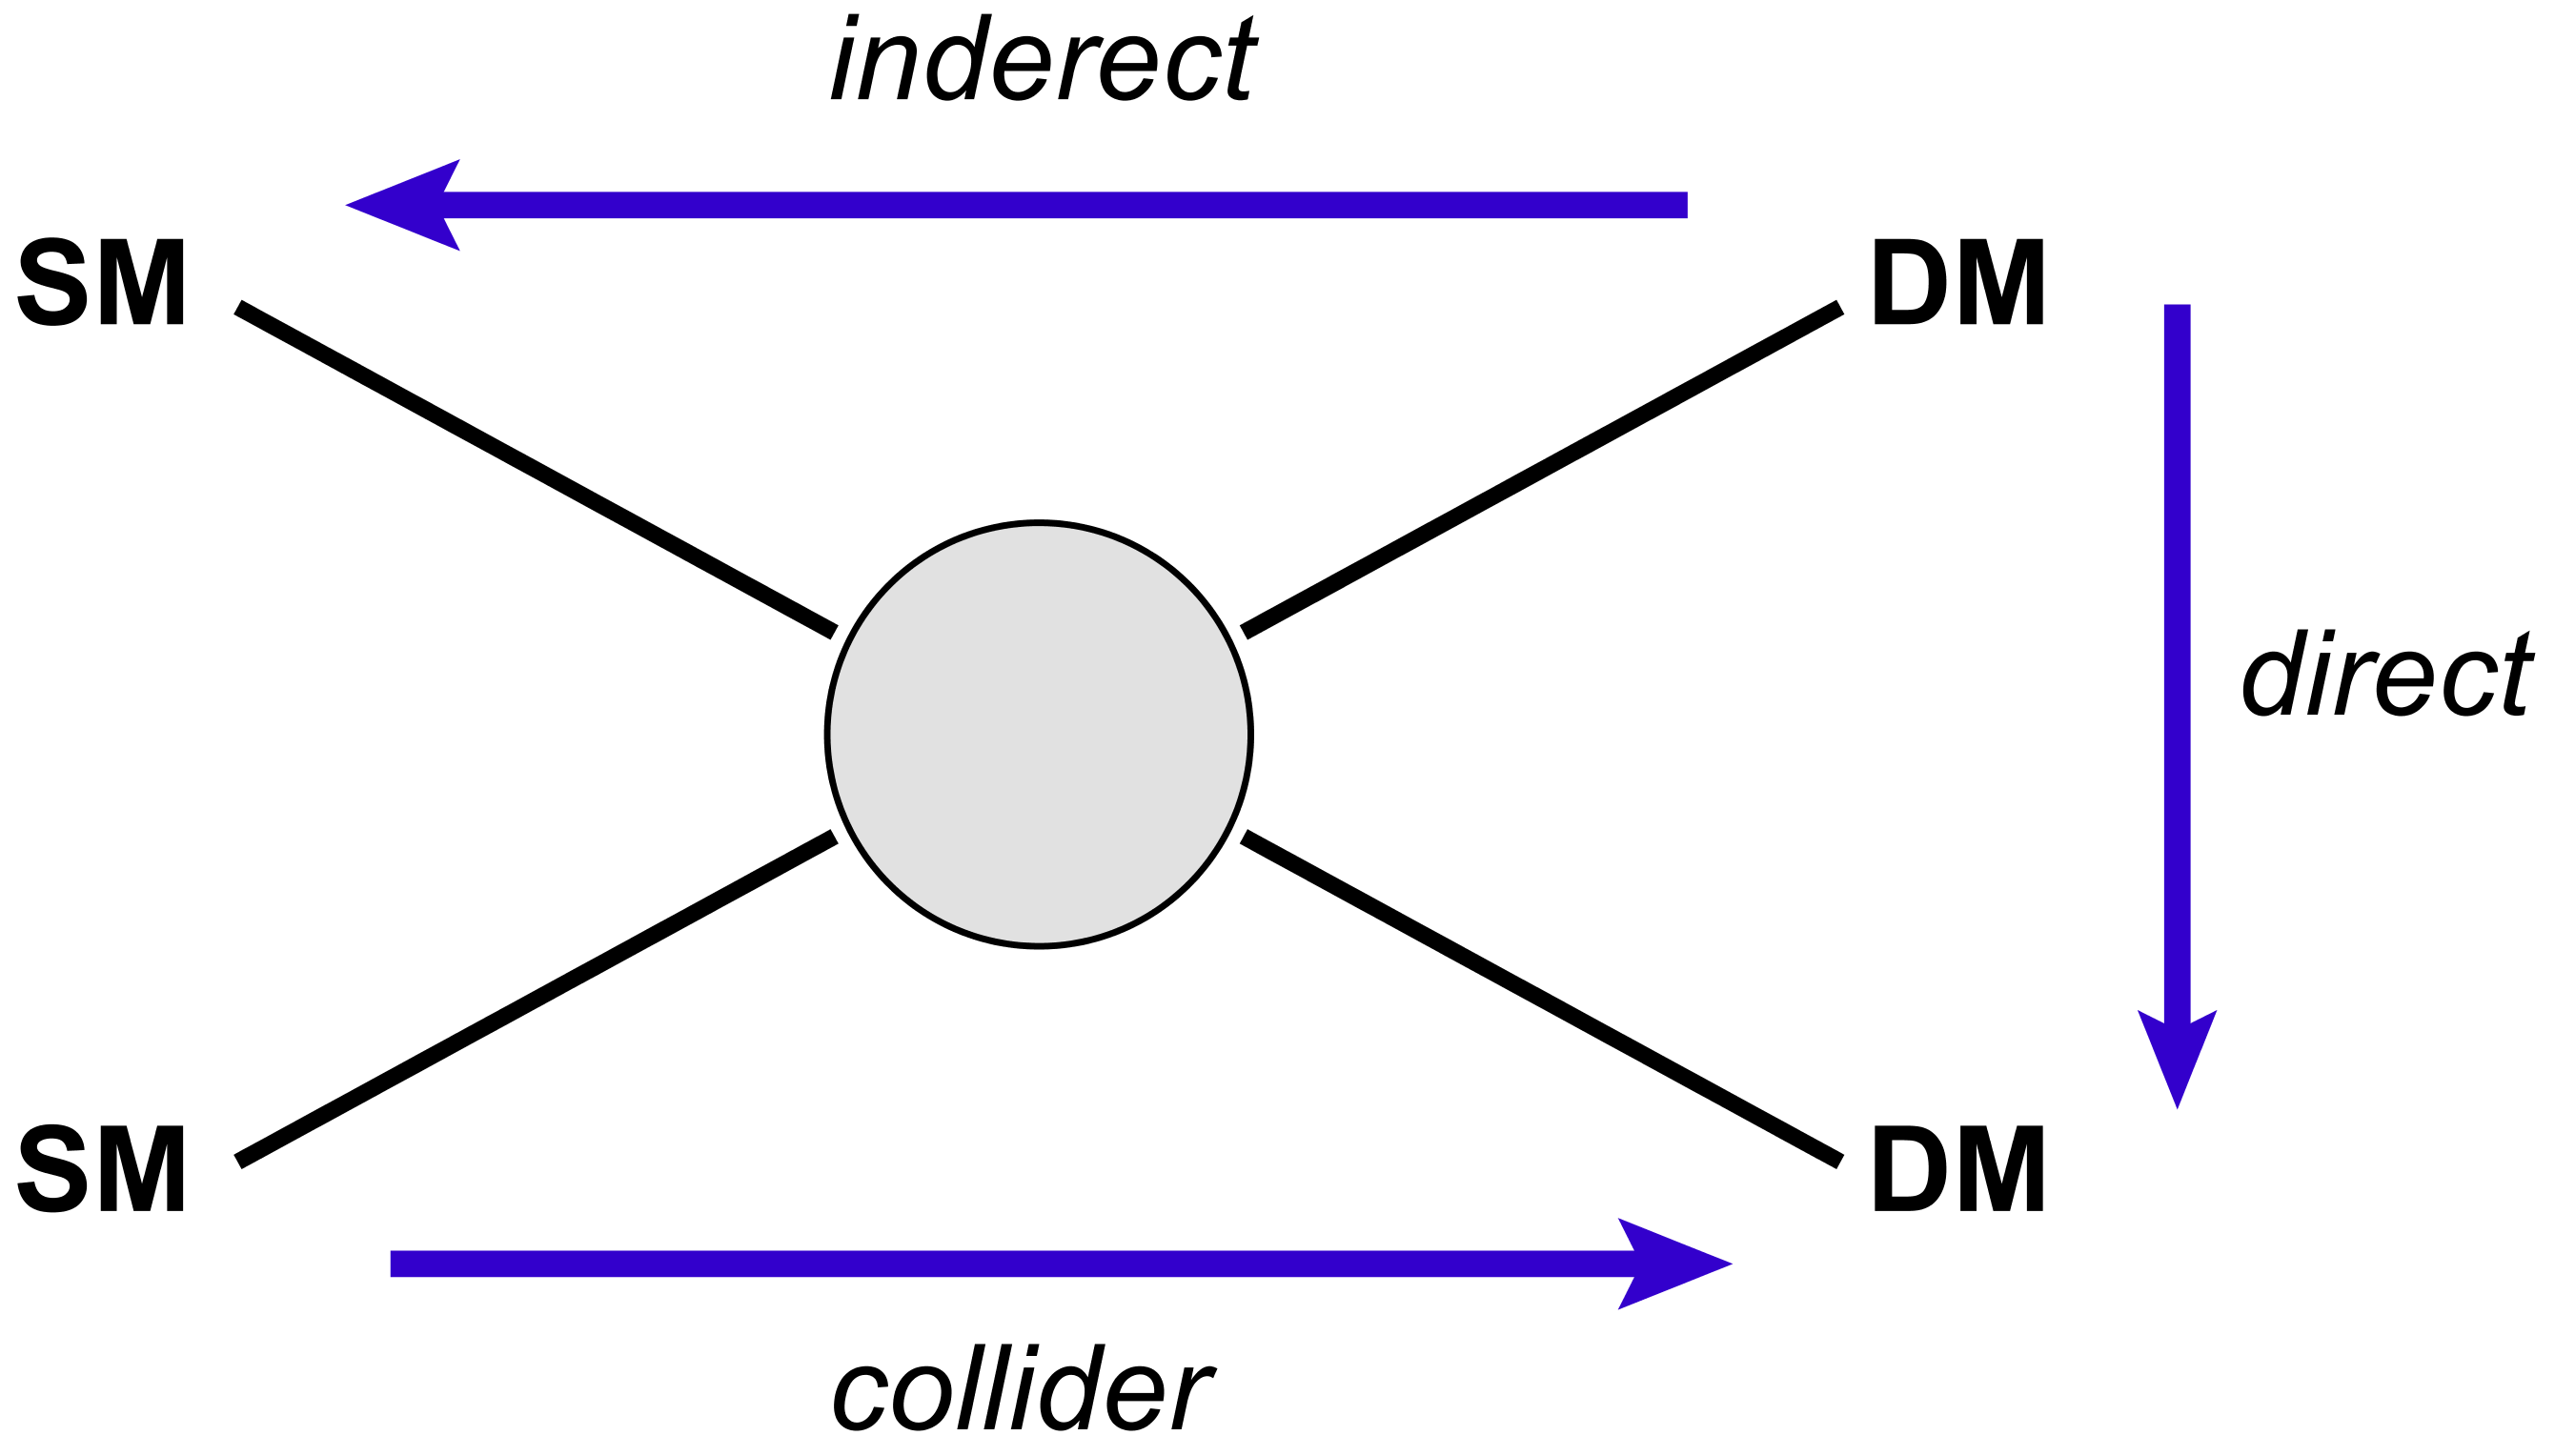
\includegraphics[width=0.9\textwidth]{pictures/Schem}\label{fig1}
	\caption{{\scriptsize Schematic showing the possible dark matter detection channels.}}
	
\end{figure}

\end{frame}
% ------------------------------------------------------------------------------------------------

%\begin{frame}
%\frametitle{Constrains Direct Detection}

%\begin{figure}[!tbp]
%	\centering
%	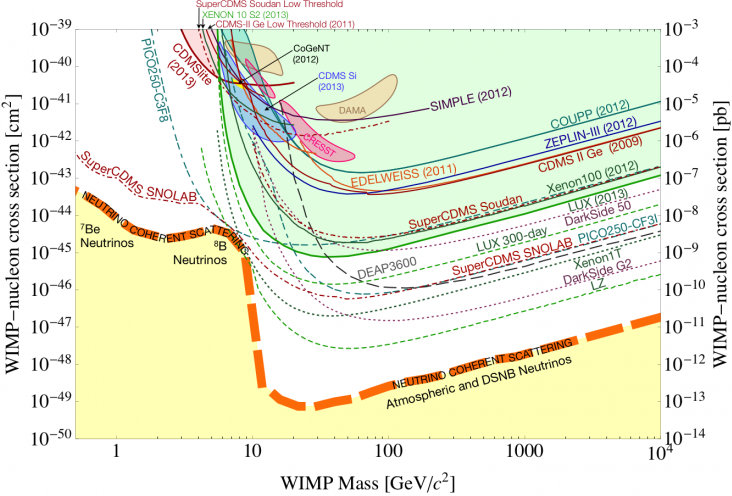
\includegraphics[width=0.9\textwidth]{pictures/WIPMS}\label{fig:f1}
%	\caption{{\scriptsize The predicted WIMP-nucleon scattering cross section as a function of WIMP mass.[APS Physics 6, 136] }}
	
%\end{figure}

%\end{frame}

% ------------------------------------------------------------------------------------------------

\section{Model}
\begin{frame}
\frametitle{Model}

\begin{textblock*}{1\linewidth}(0.25\linewidth,0.25\linewidth) % {block width} (coords)
 {\centering The Lagrangian of the model reads}
 \begin{equation}\nonumber
 \mathcal{L} = \mathcal{L}_{SM} +  m_F \bar{F}F + ( Y_\ell S \bar{F}\ell_R + {\rm h.c.} ) + V(S,H)~;
 \end{equation}\label{EQ}
 
  $m_F$ singlet fermion mass parameter, $\ell_R$ are the SM right-handed lepton fields, $Y_\ell$ 
 are the Yukawa couplings. The contribution to the scalar potential is given by
 
 \begin{equation}\nonumber
 V(S,H) = \frac{m_S^2}{2} S^2 + \frac{\lambda_S}{4} S^4 + \lambda_{SH} S^2|H|^2 ~,
 \end{equation}
 
 with scalar mass parameter $m_S$ and quartic couplings $\lambda_{S}$ and $\lambda_{SH}$.
 
\end{textblock*}


\end{frame}
% ------------------------------------------------------------------------------------------------
% ------------------------------------------------------------------------------------------------

\begin{frame}
\frametitle{Model}

\begin{textblock*}{1\linewidth}(0.25\linewidth,0.25\linewidth) % {block width} (coords)
	{\justify

	We focus on scenarios where the vector-like portal for DM annihilation is dominant and, therefore, we set initially.
	\begin{equation}\nonumber
	\lambda_{SH}=0;
	\end{equation}
	 
	also we assume that the DM candidate does not couples to the electron.
	\begin{equation}\nonumber
	Y_{e}=0;
	\end{equation}
	
	the remaining parameters, $Y_{\mu}$,$Y_{\tau}$ ,  $m_S$ and  $m_F$ are allowed to vary freely.
	
	Also we are searching into the compress mass regime 
	
		\begin{equation}\nonumber
		 \Delta m=m_{F}-m_S\lesssim 50\ \text{GeV}
		\end{equation}
	}
\end{textblock*}


\end{frame}
% ------------------------------------------------------------------------------------------------

\begin{frame}
\frametitle{Creation of DM in the Early Universe}

\begin{figure}[!tbp]
	\centering
	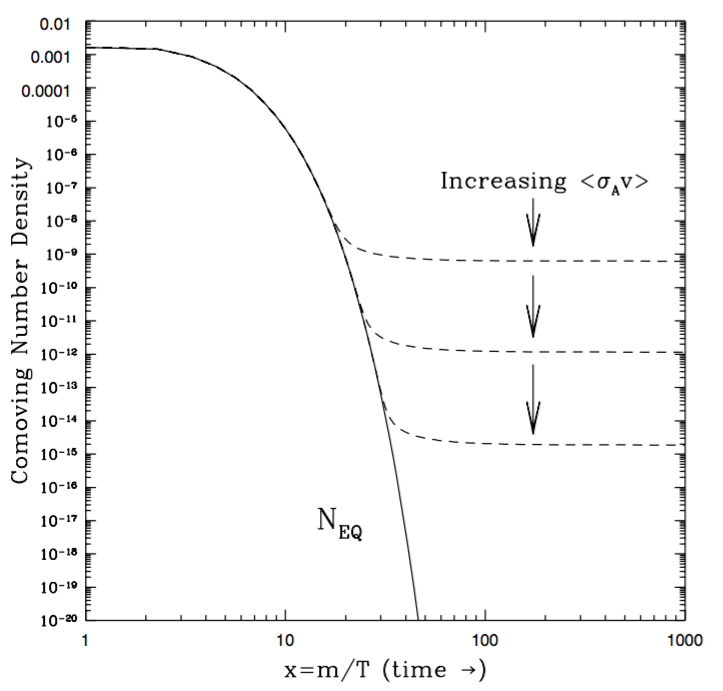
\includegraphics[width=0.7\textwidth]{pictures/FrizzOut}\label{fig2}
	\caption{{\scriptsize Equilibrium (solid curve) and relic abundance (dashed curve) of WIMP particles. Figure is taken from 	arXiv:hep-ph/9506380}}
	
\end{figure}

\end{frame}
% ------------------------------------------------------------------------------------------------

\section{Collider searches for DM}
\begin{frame}
\frametitle{Collider searches for DM}

\begin{alertblock}{Signals}
	\begin{enumerate}
		\item Cascades of heavier particles to the DM candidate and SM.
		\item[]
		\item DM production in association with other SM particles,	
	\end{enumerate}
\end{alertblock}

\end{frame}
% -------------------------------------------------------------------------

\begin{frame}
\frametitle{Experimental Signature}

\begin{textblock*}{0.5\linewidth}(0.75\linewidth,0.2\linewidth) % {block width} (coords)

\begin{figure}[!tbp]
	\centering
	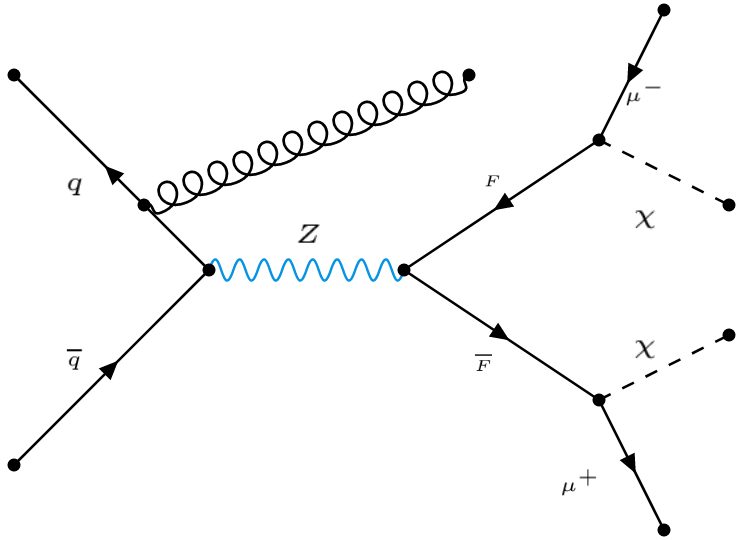
\includegraphics[width=1\textwidth]{pictures/DYVLF}\label{fig:f1}
	\caption{{\scriptsize Pair-production of vector-like fermions ($p p \to F^- F^+ $),
	in a Drell-Yan process, followed by their decay into a lepton and the DM particle ($F^- \to \ell^- S +\rm{\ h.c.},\ \ell=e,\mu,\tau$ )}}
	
\end{figure}
\end{textblock*}

\begin{textblock*}{0.46 \linewidth}(0.25\linewidth,0.25\linewidth) % {block width} (coords)
{\small {\justify The simplest production and decay process at the LHC
is pair-production of vector-like fermions,
followed by their subsequent decay to a lepton and the DM scalar.

This process leads to the signature opposite sign leptons plus missing energy.


}}
\end{textblock*}

\end{frame}
% ------------------------------------------------------------------------------------------------
\begin{frame}
\frametitle{Parameter Region}

\begin{figure}[!tbp]
	\centering
	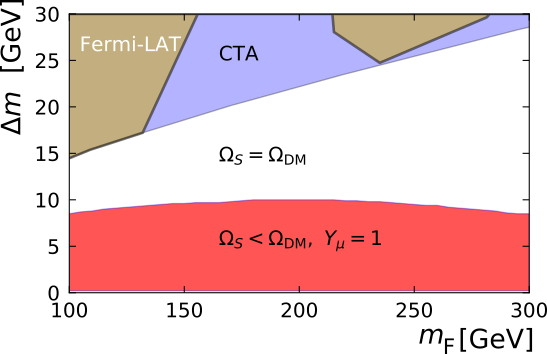
\includegraphics[width=0.9\textwidth]{pictures/PS}\label{fig1}
	\caption{{\scriptsize $m_F$ vs $\Delta m$. The brown upper region is excluded by Fermi-LAT H.E.E.S, while the combined upper region with light and magenta are the prospects for Cherenkov Telescope Array. }}
	
\end{figure}


\end{frame}
% ------------------------------------------------------------------------------------------------
% ------------------------------------------------------------------------------------------------

\section{Remarks}
\begin{frame}
\frametitle{Remarks}

\begin{exampleblock}{}
	
	\begin{enumerate}

		\item Although the model have been analyzed. there is still the region of the parameter space ($\Delta m=m_{F}-m_S\lesssim 50\ \text{GeV}$) with exclusion potential.
		\item The full dark matter content may be explained either by freeze-out at higher redshifts, or by another dark matter content.
		\item  We can obtain exclusion sensitivity over a large region of parameter has not yet been covered by any other search.
	\end{enumerate}

\end{exampleblock}

\end{frame}
% ------------------------------------------------------------------------------------------------



% ------------------------------------------------------------------------------------------------

\ThankYouFrame

% ------------------------------------------------------------------------------------------------

\end{document}
